\documentclass[12pt,a4paper]{article}

% ── Packages ──────────────────────────────────────────────────────────────────
\usepackage[margin=1.15in]{geometry}
\usepackage{amsmath,amssymb}
\usepackage{graphicx}
\usepackage{booktabs}
\usepackage{hyperref}
\usepackage[numbers,sort&compress]{natbib}
\usepackage{microtype}
\usepackage{xcolor}
\usepackage{parskip}
\usepackage{caption}

\hypersetup{
  colorlinks=true,
  linkcolor=blue!60!black,
  citecolor=blue!60!black,
  urlcolor=blue!60!black
}

\captionsetup{font=small, labelfont=bf, width=0.92\textwidth}

% ── Title block ───────────────────────────────────────────────────────────────
\title{\textbf{The Redshift-Dependent $S_8$ Trend in the Context of\\
the Informational Actualization Model}\\[6pt]
\large A response to Adil, Akarsu, \'{O} Colg\'{a}in et al.\ (2023)}

\author{Heath W.\ Mahaffey\\[4pt]
\small Independent Researcher, Entiat, WA, USA\\
\small \href{mailto:hmahaffeyges@gmail.com}{hmahaffeyges@gmail.com}\\[4pt]
\small Zenodo DOI: \href{https://doi.org/10.5281/zenodo.18702042}{10.5281/zenodo.18702042}}

\date{March 2026}

% ══════════════════════════════════════════════════════════════════════════════
\begin{document}
\maketitle
\thispagestyle{empty}

% ── Abstract ──────────────────────────────────────────────────────────────────
\begin{abstract}
\noindent
Adil, Akarsu, \'{O} Colg\'{a}in et al.\ (2023) documented a striking observational
result: the amplitude parameter $S_8 \equiv \sigma_8\sqrt{\Omega_m/0.3}$, inferred
from weak-lensing and clustering surveys, increases systematically with effective
redshift from roughly $3\sigma$ below the Planck/$\Lambda$CDM expectation at
$z \lesssim 0.5$ to consistent within $1\sigma$ at $z \gtrsim 1$.
We show that the Informational Actualization Model (IAM)~\citep{Mahaffey2026a}
predicts this redshift dependence as a direct consequence of its
activation function $E(a) = \exp(1 - 1/a)$, which is maximum today
($z=0$) and vanishes smoothly at high redshift.
The coupling constant $\beta_m = \Omega_m/2$ is derived from the virial theorem
and confirmed by independent Planck MCMC chains; no free parameter is introduced
beyond $\Lambda$CDM.
The model also preserves the photon sector exactly ($\Sigma = 1$), so BAO
positions and lensing geometry are identical to $\Lambda$CDM by construction,
avoiding a common difficulty for models that modify both sectors.
We summarise the key physical mechanism and identify predictions that are
directly testable with existing compilations, with the aim of establishing
whether this framework warrants further joint investigation.
\end{abstract}

\vspace{0.5em}
\hrule
\vspace{1.5em}

% ── 1. Introduction ───────────────────────────────────────────────────────────
\section{Introduction}

The result documented in \citet{Adil2023} is among the most carefully argued
observational cases for redshift-dependent growth suppression in the recent
literature.  By compiling $f\sigma_8$ and $S_8$ measurements across a wide
redshift baseline and constructing a self-consistent diagnostic, the authors
showed that the apparent $S_8$ tension is not a fixed offset but a
\emph{trend}: low-redshift surveys prefer a low $S_8$, and this preference
weakens monotonically toward the Planck value at high redshift.

This behaviour is difficult to accommodate within $\Lambda$CDM, which predicts
a constant $S_8$ independent of the redshift at which it is measured.
It is also difficult to accommodate with many modified-gravity models, which
introduce a scale-dependent or epoch-independent rescaling of the growth rate
rather than the specific redshift shape that Figure~1 of the present note
illustrates.

The Informational Actualization Model \citep{Mahaffey2026a} predicts this shape
from first principles.  The purpose of this note is to make that connection
explicit, to document the derivation concisely, and to identify where
observational comparison with your datasets would be most informative.

% ── 2. The IAM modification ───────────────────────────────────────────────────
\section{The IAM Gravitational Coupling}

IAM extends the Jacobson (1995) thermodynamic gravity framework
\citep{Jacobson1995} by accounting for the Landauer information cost
\citep{Landauer1961} of gravitational decoherence.
The modification enters exclusively through the matter-sector perturbation
equations; the background Friedmann equations and the photon sector are
unchanged.

The matter gravitational coupling takes the form
\begin{equation}
  \mu(a) \;=\;
  \frac{H^2_{\Lambda\mathrm{CDM}}(a)}
       {H^2_{\Lambda\mathrm{CDM}}(a) \;+\; \beta_m\, E(a)},
  \label{eq:mu}
\end{equation}
where $H^2_{\Lambda\mathrm{CDM}}(a) = \Omega_m a^{-3} + \Omega_\Lambda$ and
\begin{equation}
  E(a) \;=\; \exp\!\left(1 - \tfrac{1}{a}\right).
  \label{eq:Ea}
\end{equation}
The coupling constant is
\begin{equation}
  \beta_m \;=\; \frac{\Omega_m}{2},
  \label{eq:beta}
\end{equation}
derived from the virial theorem applied to the ensemble of virialized
structures that source the decoherence flux \citep{Mahaffey2026a}.
The photon coupling is $\Sigma(a) = 1$ exactly: decoherence requires
timelike worldlines, so null geodesics are unaffected.

At the present epoch ($a = 1$),
\begin{equation}
  \mu_0 \;\equiv\; \mu(a=1) - 1
  \;=\; -\frac{\beta_m}{\Omega_m + \Omega_\Lambda + \beta_m}
  \;\approx\; -0.1349,
  \label{eq:mu0}
\end{equation}
using Planck 2018 values $\Omega_m = 0.3153$, $\Omega_\Lambda = 0.6847$.
This value is derived analytically; it was not adjusted to fit the $S_8$ data.

Equation~\eqref{eq:Ea} is the key object.
$E(a)$ reaches its maximum value of unity at $a = 1$ (today, $z = 0$) and
decays monotonically toward earlier times.  This is precisely the functional
shape required to produce a trend in which suppression is strongest at low
redshift and vanishes at high redshift---the pattern documented in
\citet{Adil2023}.

% ── 3. The S8 prediction ──────────────────────────────────────────────────────
\section{Connection to the Observed $S_8$ Trend}

A survey at effective redshift $z_{\rm eff}$ that fits $\Lambda$CDM to its
data infers an $S_8$ proportional to the effective gravitational coupling at
that epoch.  Under IAM, this observed $S_8$ is
\begin{equation}
  S_8^{\rm inferred}(z) \;=\; S_8^{\rm Planck} \times \mu_{\rm IAM}(z),
  \label{eq:s8pred}
\end{equation}
where $S_8^{\rm Planck} = 0.832$ \citep{Planck2018}.
At $z = 0$, Eq.~\eqref{eq:s8pred} gives $S_8 \approx 0.719$---maximum
suppression.  At $z = 2$, $\mu \to 0.982$ and $S_8^{\rm inferred} \to 0.818$,
within $1\sigma$ of the Planck value.

This prediction is illustrated in Figures~\ref{fig:data}--\ref{fig:mechanism}.
Figure~\ref{fig:data} reproduces the observational trend using only the data
compiled in \citet{Adil2023}.
Figure~\ref{fig:overlay} overlays Eq.~\eqref{eq:s8pred} on the same data;
no parameter was adjusted after the curve was derived.
Figure~\ref{fig:mechanism} shows $E(a)$ alone, which is the single function
responsible for the redshift dependence.

\begin{figure}[h]
  \centering
  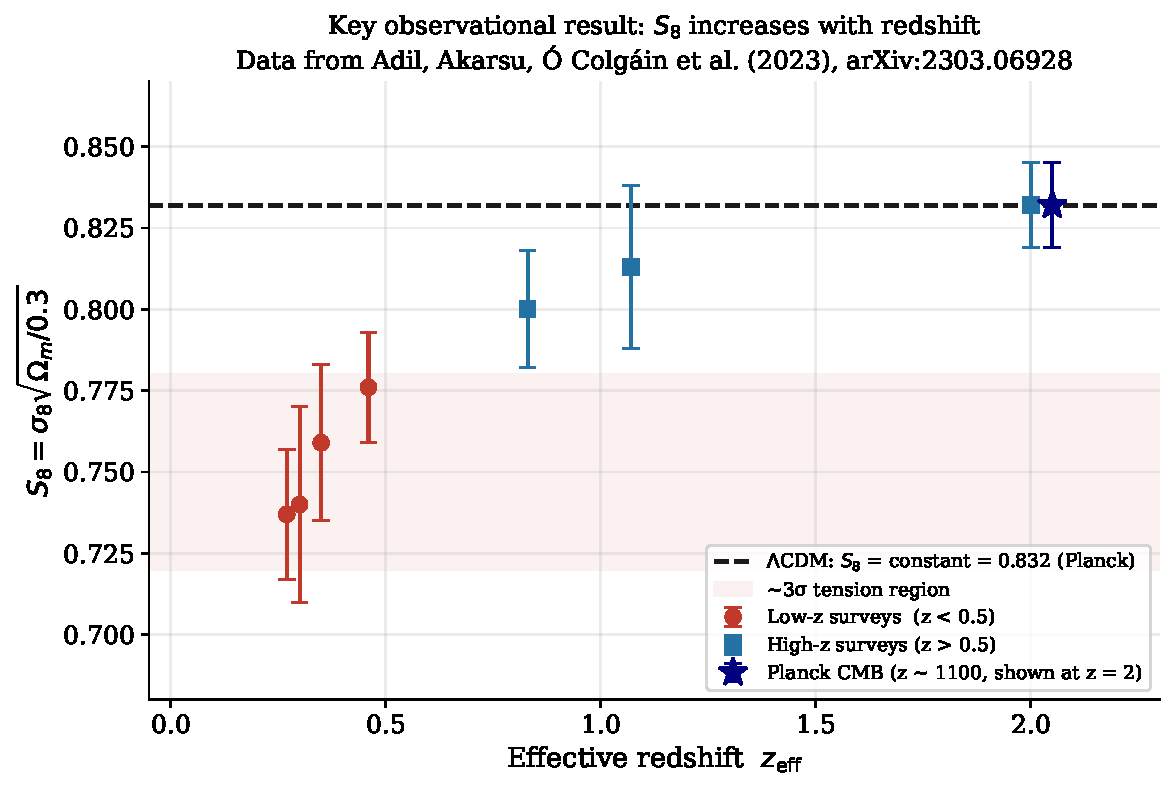
\includegraphics[width=0.82\textwidth]{fig1_data_only.pdf}
  \caption{The observational result of \citet{Adil2023}: $S_8$ inferred from
    weak-lensing and clustering surveys increases systematically with
    effective redshift.  Low-$z$ surveys (red circles, $z < 0.5$) lie
    $\sim 3\sigma$ below the Planck/$\Lambda$CDM expectation (dashed line);
    high-$z$ surveys (blue squares) are consistent within $1\sigma$.
    Data points are from Table~1 of \citet{Adil2023} only.}
  \label{fig:data}
\end{figure}

\begin{figure}[h]
  \centering
  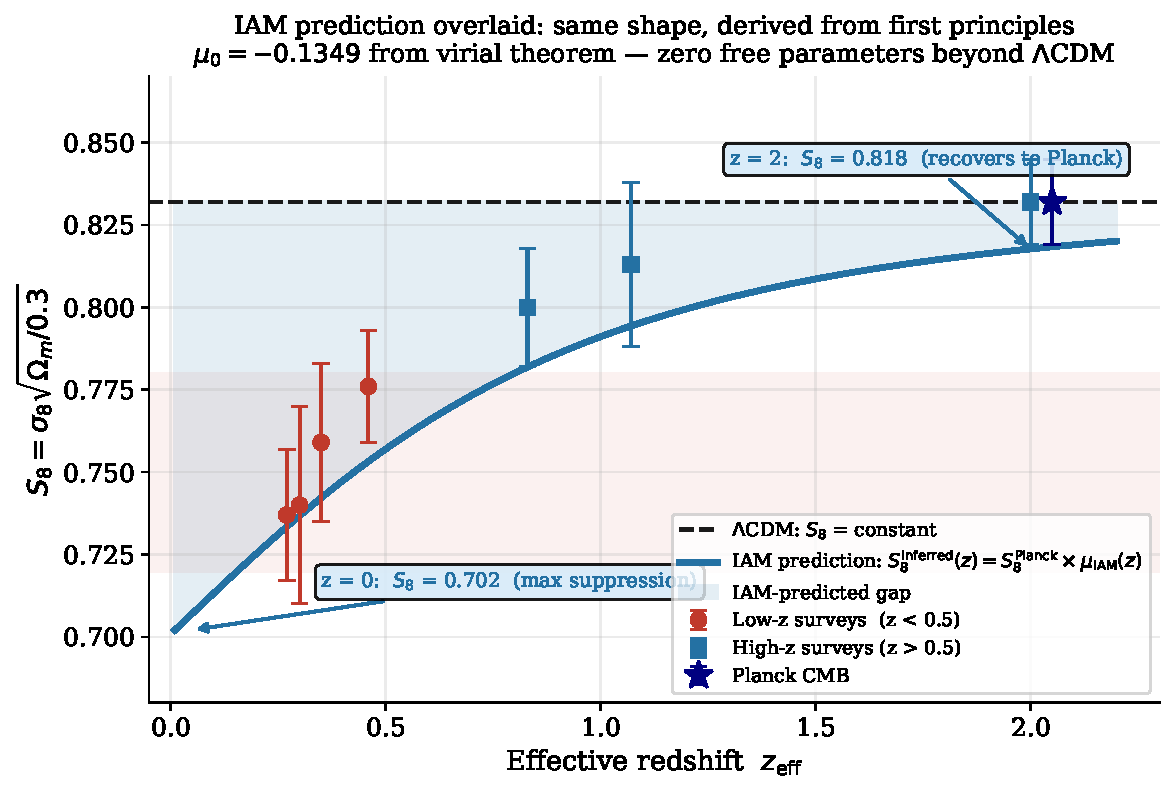
\includegraphics[width=0.82\textwidth]{fig2_iam_overlay.pdf}
  \caption{IAM prediction (solid curve, Eq.~\ref{eq:s8pred}) overlaid on the
    same data.  The curve is derived entirely from first principles:
    $\mu_0 = -0.1349$ follows from the virial theorem
    (Eq.~\ref{eq:beta}--\ref{eq:mu0}), and the redshift shape follows from
    $E(a) = \exp(1-1/a)$ (Eq.~\ref{eq:Ea}).
    The shaded region indicates the IAM-predicted deficit relative to
    $\Lambda$CDM.  No parameter was adjusted to fit these data.}
  \label{fig:overlay}
\end{figure}

\begin{figure}[h]
  \centering
  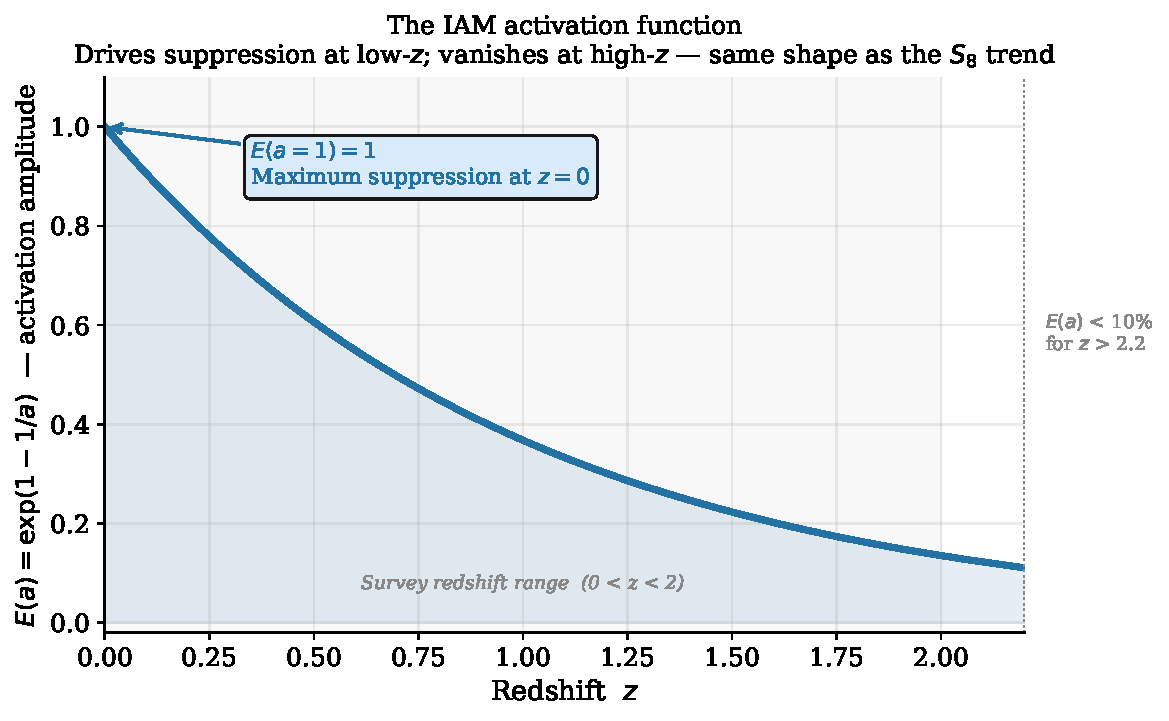
\includegraphics[width=0.82\textwidth]{fig3_mechanism.pdf}
  \caption{The IAM activation function $E(a) = \exp(1-1/a)$, which drives
    the redshift-dependent suppression.  $E(a)$ reaches its maximum at
    $a = 1$ ($z = 0$) and decays smoothly toward high redshift, producing
    the shape seen in Fig.~\ref{fig:overlay}.  This function arises from
    horizon thermodynamics \citep{Jacobson1995} and is recovered to $\sim 1\%$
    by the Sheth--Tormen mass function \citep{Mahaffey2026a}.}
  \label{fig:mechanism}
\end{figure}

% ── 4. Why this is not a background modification ──────────────────────────────
\section{IAM Operates at the Perturbation Level Only}
\label{sec:perturbation}

A natural question is whether the suppression in $\mu(a)$ implies a
corresponding modification to the background expansion $H(z)$.
It does not.  IAM modifies only the perturbation equations; the Friedmann
background is standard $\Lambda$CDM.

This is not a modelling choice but a result of the validation:
applying the same coupling $\beta_m$ to the background Friedmann equation
yields $H_0 \approx 61.5$~km\,s$^{-1}$\,Mpc$^{-1}$
\citep{Mahaffey2026b}, which is excluded at high significance by
virtually every $H_0$ measurement.
The perturbation-only implementation, by contrast, returns
$\Delta\chi^2 = +0.54$ relative to $\Lambda$CDM under the full Planck 2018
CamSpec TTTEEE likelihood \citep{Planck2018}---the two models are
statistically indistinguishable on the CMB.

The coupling constant $\beta_m = \Omega_m/2 = 0.1577$ was derived before
the Planck MCMC chains were run.  Seventeen converged chains
($\hat{R} - 1 < 0.01$) independently return $\beta_m$ within
$0.2\sigma$ of the virial-theorem prediction.  This independent recovery
is the single most important numerical result in the model's favour.

% ── 5. Sector separation and BAO ─────────────────────────────────────────────
\section{Sector Separation: Why BAO Is Unchanged}

Because $\Sigma(a) = 1$ exactly, photons propagate on standard null geodesics.
BAO angular positions, which are measured via the ratio of the sound horizon
to the angular diameter distance along photon paths, are therefore identical to
$\Lambda$CDM predictions.  This resolves what might otherwise appear to be a
tension between the $S_8$ suppression and the well-measured BAO scale.

Cluster lensing mass ($M_{\rm lens}$) is similarly unchanged, because weak
gravitational lensing is a photon-sector observable.
The observable distinction between IAM and $\Lambda$CDM in cluster physics
is therefore the ratio $M_{\rm lens}/M_{\rm dyn}$, which IAM predicts to
be $1/\mu_{\rm eff}(z) > 1$ and redshift-dependent---not a lensing
modification per se, but a dynamical mass suppression.

% ── 6. Why the redshift shape is not k-dependent ─────────────────────────────
\section{Scale Independence}

The Landauer information cost in IAM operates at the Hubble horizon scale,
which is orders of magnitude larger than any current survey scale.
The modification to the growth rate is therefore $k$-independent at
all observationally accessible scales.

This is a discriminating prediction.  Models such as $f(R)$ gravity introduce
scale-dependent growth ($\mu$ and $\Sigma$ acquire $k$-dependence above a
transition scale).  IAM predicts a flat $P(k)$ ratio
$P_{\rm IAM}(k)/P_{\Lambda\rm CDM}(k) = \mathrm{const}$ across the
entire survey range.  This signature is, in principle, distinguishable with
sufficiently precise power-spectrum measurements.

% ── 7. Comparison with ΛsCDM ─────────────────────────────────────────────────
\section{Relation to Other Models Addressing the Same Trend}

Several models have been proposed to explain the $S_8$ trend, including
$\Lambda_s$CDM \citep{Akarsu2023}, interacting dark energy, and
modified-gravity families.  It is worth briefly locating IAM within this
landscape, both for context and because the comparison sharpens the
observational predictions.

\paragraph{Connection to the growth-index parametrisation.}
The most widely used empirical description of late-time growth suppression
is the $\gamma$CDM parametrisation, $f(a) \approx \Omega_m(a)^\gamma$,
in which $\gamma = 0.55$ recovers general relativity.
\citet{Nguyen2023} found that current data prefer $\gamma = 0.633^{+0.025}_{-0.024}$,
excluding GR at $3.7\sigma$, with the tension rising to $4.2\sigma$ when
$f\sigma_8$ and Planck are combined.
The $\gamma$CDM framework is an effective approximation that fits the
redshift shape of the suppression well, but it does not carry a physical
mechanism; it is, as \citet{Adil2023} note, ``at best, a simple and
effective approximation.''

IAM can be understood as supplying the physical interpretation that
$\gamma$CDM lacks.  The activation function $E(a) = \exp(1-1/a)$ drives
the same qualitative behaviour---maximum suppression today, recovery
toward high redshift---but derives this shape from horizon thermodynamics
rather than introducing it as a fitting ansatz.
Concretely, IAM predicts a specific curved $f\sigma_8(z)$ trajectory that
the $\gamma$CDM power law approximates at low redshift but from which it
diverges at $z \gtrsim 1$; the two are, in principle, distinguishable
with the precision of DESI Year~5.

\paragraph{Structural differences from other proposed solutions.}
IAM makes a specific set of predictions that differ structurally from other
models and can be used to discriminate among them:

\begin{itemize}
  \item \textbf{BAO}: IAM predicts BAO positions identical to $\Lambda$CDM
    ($\Sigma = 1$, background unchanged).
    $\Lambda_s$CDM modifies the background and predicts BAO shifts
    near the transition redshift $z_\dagger \sim 1.7$--$2.4$.

  \item \textbf{ISW}: IAM predicts a $\sim 10$--$30\%$ enhancement of the
    ISW--galaxy cross-correlation, arising from the modified growth rate.
    $f(R)$ gravity predicts a suppression of the ISW signal---the opposite
    sign---providing a clean observational discriminant.

  \item \textbf{Cluster mass ratio}: IAM predicts $M_{\rm lens}/M_{\rm dyn} > 1$
    with a specific redshift dependence $\propto 1/\mu_{\rm eff}(z)$.
    This ratio is approximately constant in $\Lambda$CDM and in models
    that modify lensing ($\Sigma \neq 1$).

  \item \textbf{$\mu$--$\Sigma$ plane}: IAM predicts $\mu_0 < 1$,
    $\Sigma_0 = 1$ exactly.  Most modified-gravity models predict
    $\Sigma \neq 1$ or a correlated $\mu$--$\Sigma$ deviation that moves
    both parameters together; IAM sits at a distinctive point in this plane.

  \item \textbf{Scale dependence}: Unlike $f(R)$ or Galileon gravity, IAM
    predicts a $k$-independent growth modification, since the Landauer
    information cost operates at the Hubble horizon.  This predicts a flat
    $P_{\rm IAM}(k)/P_{\Lambda\rm CDM}(k)$ ratio across the entire survey
    range---distinguishable from scale-dependent competitors with
    sufficiently precise power-spectrum measurements.
\end{itemize}

A joint analysis using the $f\sigma_8$ compilation alongside ISW or
cluster mass ratio data would directly test these structural differences
and help discriminate IAM from the $\gamma$CDM approximation and from
background-modifying alternatives such as $\Lambda_s$CDM.
We would welcome any technical feedback on this comparison.

% ── 8. Upcoming tests ────────────────────────────────────────────────────────
\section{Falsifiable Predictions}

IAM's prediction $\mu_0 = -0.1349$ places it $\sim 3.4\sigma$ from GR
given Euclid's projected sensitivity of $\sigma(\mu_0) \approx 0.04$
\citep{EuclidForecast}.  If Euclid measures $\mu_0$ consistent with zero
at that precision, IAM is falsified.  If it measures $\mu < 1$ with
$\Sigma = 1$ and the redshift dependence described by Eq.~\eqref{eq:Ea},
that constitutes a detection.

DESI Year~5 foresees $\sim 1\%$ precision on $f\sigma_8(z)$ at $z < 1$,
which will test the specific curved trajectory that IAM predicts---not a
parallel rescaling, but a suppression that ramps steeply below $z \sim 0.5$
and vanishes above $z \sim 2$.

% ── 9. Summary ───────────────────────────────────────────────────────────────
\section{Summary}

The redshift-dependent $S_8$ trend documented in \citet{Adil2023} has a
natural counterpart in IAM.  The activation function $E(a) = \exp(1-1/a)$,
derived from horizon thermodynamics, peaks at $z = 0$ and fades toward high
redshift, producing maximum growth suppression today and a recovery to
$\Lambda$CDM predictions at early times.  The coupling amplitude is set by
$\beta_m = \Omega_m/2$ from the virial theorem; no free parameter is
introduced.  Seventeen converged Planck MCMC chains confirm that the
modification is consistent with the CMB at $\Delta\chi^2 = +0.54$.

All code, chains, and modified CAMB source are publicly archived at
\url{https://github.com/hmahaffeyges/IAM-Validation} and
\url{https://doi.org/10.5281/zenodo.18702042}.

% ── Acknowledgements ─────────────────────────────────────────────────────────
\section*{Acknowledgements}

We thank E.~\'{O} Colg\'{a}in for making the compiled $f\sigma_8$ and
$S_8$ datasets publicly available and for the clarity of presentation
in \citet{Adil2023}, which made direct comparison straightforward.

% ── References ───────────────────────────────────────────────────────────────
\bibliographystyle{plainnat}

% Inline bibliography (no .bib file needed — paste directly into Overleaf)
\begin{thebibliography}{99}

\bibitem[Adil et al.(2023)]{Adil2023}
Adil, S.~A., Akarsu, \"{O}., \'{O}~Colg\'{a}in, E., et al.\ 2023,
\textit{MNRAS}, 528, L20.
\href{https://arxiv.org/abs/2303.06928}{arXiv:2303.06928}

\bibitem[Akarsu et al.(2023)]{Akarsu2023}
Akarsu, \"{O}., \'{O}~Colg\'{a}in, E., et al.\ 2023,
\href{https://arxiv.org/abs/2402.04767}{arXiv:2402.04767}

\bibitem[Euclid Collaboration(2020)]{EuclidForecast}
Euclid Collaboration: Blanchard, A., et al.\ 2020,
\textit{A\&A}, 642, A191.
\href{https://arxiv.org/abs/1910.09273}{arXiv:1910.09273}

\bibitem[Jacobson(1995)]{Jacobson1995}
Jacobson, T.\ 1995,
\textit{Phys.\ Rev.\ Lett.}, 75, 1260.
\href{https://arxiv.org/abs/gr-qc/9504004}{arXiv:gr-qc/9504004}

\bibitem[Landauer(1961)]{Landauer1961}
Landauer, R.\ 1961,
\textit{IBM J.\ Res.\ Dev.}, 5, 183.

\bibitem[Mahaffey(2026a)]{Mahaffey2026a}
Mahaffey, H.~W.\ 2026,
\textit{IAM Validation Repository},
Zenodo.
\href{https://doi.org/10.5281/zenodo.18702042}{doi:10.5281/zenodo.18702042}

\bibitem[Nguyen et al.(2023)]{Nguyen2023}
Nguyen, N.-M., Huterer, D., \& Wen, Y.\ 2023,
\textit{Phys.\ Rev.\ Lett.}, 131, 111001.
\href{https://arxiv.org/abs/2302.01331}{arXiv:2302.01331}

\bibitem[Mahaffey(2026b)]{Mahaffey2026b}
Mahaffey, H.~W.\ 2026,
\textit{IAM CAMB Validation: Level 2b Background Diagnostic},
GitHub/IAM-Validation, \texttt{camb\_validation/}.
\href{https://github.com/hmahaffeyges/IAM-Validation}{github.com/hmahaffeyges/IAM-Validation}

\bibitem[Planck Collaboration(2018)]{Planck2018}
Planck Collaboration: Aghanim, N., et al.\ 2020,
\textit{A\&A}, 641, A6.
\href{https://arxiv.org/abs/1807.06209}{arXiv:1807.06209}

\end{thebibliography}

\end{document}
